\documentclass[a4paper]{article}
\usepackage[spanish]{babel}
\usepackage[utf8]{inputenc}
\usepackage{charter}   % tipografia
\usepackage{graphicx}
\usepackage{enumerate}
\usepackage{listings}
\usepackage{color}
%\usepackage{indentfirst}
\usepackage{fancyhdr}
\usepackage{latexsym}
\usepackage{lastpage}
\usepackage[colorlinks=true, linkcolor=black]{hyperref}
%\usepackage{makeidx}
%\usepackage{float}
\usepackage{calc}
\usepackage{amsthm, amssymb}
\usepackage[nosumlimits]{amsmath} % este package hace que se vean mal los incides en las sumatorias, pero permite poner uno abajo del otro en la ecuacon de los L de laagrange

\usepackage{subfig}

\usepackage{amsfonts}

%\usepackage{sectsty}
%\usepackage{charter}
%\usepackage{wrapfig}
%\usepackage{listings}
%\lstset{language=C}
\definecolor{gray}{gray}{0.5}
\definecolor{light-gray}{gray}{0.95}
\definecolor{orange}{rgb}{1,0.5,0}

\usepackage{color} % para snipets de codigo coloreados
\usepackage{fancybox}  % para el sbox de los snipets de codigo

\definecolor{litegrey}{gray}{0.94}

% \newenvironment{sidebar}{%
% 	\begin{Sbox}\begin{minipage}{.85\textwidth}}%
% 	{\end{minipage}\end{Sbox}%
% 		\begin{center}\setlength{\fboxsep}{6pt}%
% 		\shadowbox{\TheSbox}\end{center}}
% \newenvironment{warning}{%
% 	\begin{Sbox}\begin{minipage}{.85\textwidth}\sffamily\lite\small\RaggedRight}%
% 	{\end{minipage}\end{Sbox}%
% 		\begin{center}\setlength{\fboxsep}{6pt}%
% 		\colorbox{litegrey}{\TheSbox}\end{center}}

\newenvironment{codesnippet}{%
	\begin{Sbox}\begin{minipage}{\textwidth}\sffamily\small}%
	{\end{minipage}\end{Sbox}%
		\begin{center}%
		\colorbox{litegrey}{\TheSbox}\end{center}}



\usepackage{fancyhdr}
\pagestyle{fancy}

%\renewcommand{\chaptermark}[1]{\markboth{#1}{}}
\renewcommand{\sectionmark}[1]{\markright{\thesection\ - #1}}

\fancyhf{}

\fancyhead[LO]{Sección \rightmark} % \thesection\ 
\fancyfoot[LO]{\small{nombre, nombre, nombre}}
\fancyfoot[RO]{\thepage}
\renewcommand{\headrulewidth}{0.5pt}
\renewcommand{\footrulewidth}{0.5pt}
\setlength{\hoffset}{-0.8in}
\setlength{\textwidth}{16cm}
%\setlength{\hoffset}{-1.1cm}
%\setlength{\textwidth}{16cm}
\setlength{\headsep}{0.5cm}
\setlength{\textheight}{25cm}
\setlength{\voffset}{-0.7in}
\setlength{\headwidth}{\textwidth}
\setlength{\headheight}{13.1pt}

\renewcommand{\baselinestretch}{1.1}  % line spacing


% \setcounter{secnumdepth}{2}
\usepackage{underscore}
\usepackage{caratulaV}
\usepackage{url}
\usepackage{float}

%\usepackage{makeidx}


% \setcounter{secnumdepth}{2}
\usepackage{underscore}
\usepackage{alltt}
\usepackage{tikz}
\usepackage{color}
% \usepackage{gnuplottex}
\usepackage{verbatim}
\usepackage{algorithm}
\usepackage{algpseudocode}

\definecolor{dkgreen}{rgb}{0,0.6,0}
\definecolor{gray}{rgb}{0.5,0.5,0.5}
\definecolor{mauve}{rgb}{0.58,0,0.82}

\lstset{frame=tb,
  language=Python,
  aboveskip=3mm,
  belowskip=3mm,
  showstringspaces=false,
  columns=flexible,
  basicstyle={\small\ttfamily},
  keywordstyle=\color{blue},
  commentstyle=\color{dkgreen},
  stringstyle=\color{mauve},
  breaklines=true,
  breakatwhitespace=true,
  tabsize=3,
  numbers=left,
  xleftmargin=2em,
  frame=single,
  framexleftmargin=2em,
  numbersep=5pt,                   % how far the line-numbers are from the code
  numberstyle=\small\color{gray} % the style that is used for the line-numbers
 }

\parskip = 5 pt

\newcounter{row}
\newcounter{col}

\newcommand\setrow[3]{
	\setcounter{col}{1}
	\foreach \n in {#1, #2, #3} {
	\edef\x{\value{col} - 0.5}
	\edef\y{3.5 - \value{row}}
	\node[anchor=center] at (\x, \y) {\n};
	\stepcounter{col}
	}
	\stepcounter{row}
}

\newcommand\setrowaux[7]{
	\setcounter{col}{1}
	\foreach \n in {#1, #2, #3, #4, #5, #6, #7} {
	\edef\x{\value{col} - 0.5}
	\edef\y{7.5 - \value{row}}
	\node[anchor=center] at (\x, \y) {\n};
	\stepcounter{col}
	}
	\stepcounter{row}
}

\newcommand\setrowauxx[4]{
	\setcounter{col}{1}
	\foreach \n in {#1, #2, #3, #4} {
	\edef\x{\value{col} - 0.5}
	\edef\y{4.5 - \value{row}}
	\node[anchor=center] at (\x, \y) {\n};
	\stepcounter{col}
	}
	\stepcounter{row}
}


\begin{document}


\thispagestyle{empty}
\materia{Métodos Numéricos}
\submateria{Primer Cuatrimestre - 2015}
\titulo{Trabajo Práctico III}
\subtitulo{Marche un telebeam Don Niembraaaaaa...}
\integrante{}{}{}
\integrante{}{}{}
\integrante{}{}{}
\integrante{}{}{}

\maketitle
\newpage


\vspace{3cm}
\tableofcontents
\thispagestyle{empty}

\newpage


\begin{comment}
\begin{codesnippet}
\begin{verbatim}

struct Pepe {

    ...

};

\end{verbatim}
\end{codesnippet}

\begin{lstlisting}
for (x = 1 to n - 2):
	xmm1  <--  img[x-1][0] , img[x][0] , img[x+1][0] , img[x+2][0]
	xmm2  <--  img[x-1][1] , img[x][1] , img[x+1][1] , img[x+2][1]
	xmm1  <--  borrarprimero(xmm1)
	xmm2  <--  borrarprimero(xmm2)
	xmm1  <--  sumapixels(xmm1)
	xmm2  <--  sumapixels(xmm2)
	for (y = 1 to n - 2): 
		xmm0  <--  xmm1
		xmm1  <--  xmm2
		xmm3  <--  img[x-1][y+1] , img[x][y+1] , img[x+1][y+1] , img[x+2][y+1]
		xmm3  <--  borrarprimero(xmm3)
		xmm3  <--  sumapixels(xmm3)
		xmm0  <--  xmm0 + xmm1 + xmm2
		xmm0  <--  promedio(xmm0)
		img[x][y]  <--  xmm0
	end
end
\end{lstlisting}


\begin{figure}[H]
\centering
\includegraphics[scale=0.8]{imagenes/256value.png}
\caption{Contenido de los registros utilizados para multiplicar}
\label{256value}
\end{figure}



\begin{figure}[H]
	\minipage{0.5\textwidth}
	\begin{center}
		\includegraphics[scale=0.4]{../tp2-bundle.v2/Testing/plots/all/merge-black-05--all.png}
		\caption{Rendimiento para un value de 0.5, imágenes negras.}
		\label{fig:exp1-5}
	\end{center}
	\endminipage\hfill
	\minipage{0.5\textwidth}
	\begin{center}
		\includegraphics[scale=0.4]{../tp2-bundle.v2/Testing/plots/all/merge-normal-00--all.png}
		\caption{Rendimiento para un value de 0.0, imágenes normales.}
		\label{fig:exp1-2}
	\end{center}
	\endminipage\hfill
\end{figure}


\end{comment}

\setcounter{page}{1}


\begin{abstract}

En este trabajo se utilizaran distintas técnicas para obtener un re-escalamiento de imágenes. Se utilizara vecino más cercano, interpolación de polinomios bilineal, splines cúbicos, y distintas variantes de los métodos anteriormente mencionados. Se implementaran algoritmos para los mismos, dando la posibilidad de re-escalar las imágenes en distintos tamaños(siempre mayor al original). Se llevara a cabo una experimentación con su respectivo análisis. Como las imágenes obtenidas, no contienen integramente información original, se utilizaran las métricas de Error Cuadrático Medio (ECM) y Peak to Signal Noise Ratio (PSNR) para estudiar en forma cuantitativa la calidad de las mismas. También se considerara la calidad subjetiva, y el tiempo de computo. 

\textbf{Palabras Clave}: re-escalamiento imágenes, interpolación, ECM, PSNR

\end{abstract}

\newpage

\section{Intoducción}

En el presente trabajo se nos plantea como objetivo el re-escalamiento de imágenes, específicamente ampliarlas.

Se trabajara con imágenes en escala de grises por lo que dada una imagen de mxn, contendrá mxn pixels cada uno con un valor entre 0-255.

Para ampliar las imágenes, a partir de un valor $k \in \mathbb{N}_{>0}$ insertaremos entre la fila i y la fila i +1, k filas con i = 1, ....., m -1, y de manera análoga para las columnas. De esta forma obtendremos una nueva imagen con $(m -1)*k + m$ filas y $(n -1)*k + n$ columnas.

El problema que ahora se genera es ¿que valores asignar a los pixels de las columnas y filas agregadas?. Para esto, emplearemos distintos criterios de asignación de valor a partir de ciertos métodos.

En primera instancia consideraremos el método de vecino mas cercano, para esto el valor de un píxel nuevo sera igual a aquel cuya distancia a otro píxel, en una vecindad definida, sea la mínima. En particular la vencidad tomada será de aquellos cuatro valores más cercano con respecto a los pixels originales (pixels de la imagen sin ampliar, $imagen$ $original$). 

Otro método empleado fue mediante la interpolación de polinomios, esta consiste en que dada una terna de puntos ($ x_{0} $, $ y_{0} $), ($ x_{1} $, $ y_{1} $), $ \ldots $ ($ x_{n} $, $ y_{n} $) se busca obtener un polinomio $P$ que los interpole es decir, que verifique $ p(x_{0}) =  y_{0} $, $ p(x_{1}) =  y_{1} $, $ \ldots $ $ p(x_{n}) =  y_{n} $. En general, la interpolación de una serie de puntos es usada para aproximar una función continua en un cierto intervalo. 
Dado que siempre existe un polinomio interpolador para $n+1$ puntos, de grado a lo sumo n que los interpole$^{1}$ %Burden 7 edicion teorema 3.2 pag 109
, una de la forma de obtenerlo es mediante el método de interpolación de Lagrange, el cual se basa en construir primero los polinomios $ L_{n,k} $ definidos como se indica en la ecuación~\ref{Ls}.

\begin{equation}
L_{n,k}= \prod_{\substack{i=0\\i\neq k}}^{n} \frac{(x-x_{i})}{(x_{k}-x_{i})}
\label{Ls}
\end{equation}

El polinomio de grado a lo sumo $ n $ que interpola los $ n +1 $ puntos se construye según la ecuación~\ref{lagrange}.
\begin{equation}
P(x)= \sum_{k=0}^{n}y_{k}L_{n,k}(x)
\label{lagrange}
\end{equation}
Por lo que el segundo método empleado consiste en usar interpolación bilineal entre dos puntos ($ x_{0} $, $ y_{0} $) y ($ x_{1} $, $ y_{1} $), en nuestro caso entre dos pixels, por lo que el polinomio interpolador de Lagrange sera de grado a lo sumo uno es decir, será una recta que pasa por dos puntos. En la ecuación~\ref{bilinealInter}
\begin{equation}
P(x)= L_{1,0}(x)y_{0} + L_{1,1}(x)y_{1} = \frac{x -x_{1}}{x_{0}-x_{1}}y_0 + \frac{x-x_{0}}{x_{1}-x_{0}} y_{1}
\label{bilinealInter}
\end{equation}
o equivalentemente obtenemos una formula mas clara para el mismo, donde además podemos distinguir la pendiente y la ordenada al origen.
\begin{equation}
P(x)= \frac{y_{1}-y_{0}}{x_{1}-x_{0}}(x - x_{0}) + y_{0}
\label{bilineal}
\end{equation}
Ses $f(x_i)$ = $y_i$, en nuestro caso el valor de f depende de dos puntos, por lo que el valor del píxel $p_{ij}$ se obtendrá extendiendo la ecuación~\ref{bilineal} a:
\begin{equation}
p(i, j) = \frac{f(i, j_1)-f(i,j_0)}{j_1 - j_0} + f(i,j_0)
\end{equation}
Otro de los métodos utilizados es el de splines cúbicos. Dada una función $f$ definida en $[a,b]$ y un conjunto de puntos $a=x_0<x_1<\ldots<x_n=b$ un trazador cúbico $S$ para $f$ es una función tal que en cada subintervalo $[x_j, x_{j+1}]$ con  $j=0,1,\ldots,n-1$ $S_j(x)$ es un polinomio cubico, y verifica:
\begin{itemize}
  \item $S(x_j)=f(x_j)$ $ \forall $ $j=0,1,\ldots,n$
  \item $S_{j+1}(x_{j+1})=S_j(x_{j+1})$ $ \forall $ $j=0,1,\ldots,n-2$
  \item $S_{j+1}'(x_{j+1})=S_j'(x_{j+1})$ $ \forall $ $j=0,1,\ldots,n-2$
  \item $S_{j+1}''(x_{j+1})=S_j''(x_{j+1})$ $ \forall $ $j=0,1,\ldots,n-2$
  \item Y una de las siguientes condiciones
        \begin{itemize}
                \item $S''(x_0)=S''(x_n)=0$ $ \forall $ $j=0,1,\ldots,n-2$ (condición natural)
                 \item $S'(x_0)=f'(x_0) y S'(x_n)=f'(x_n)$ (condición sujeta)
        \end{itemize}
\end{itemize}
Escribiendo a los $ S_j $ en la forma $S_j(x) = a_j + b_j(x-x_j)+c_j(x-x_j)^2+d_j(x-x_j)^3$, y planteando las condiciones anteriormente mencionadas se puede obtener un sistema lineal de $ n+1 $ ecuaciones y $ n+1 $ incógnitas, donde estas son los $ c_{j} $. En el caso de la condición natural, que fue el utilizado en este trabajo práctico, mas específicamente se obtiene:
$$
A =
\begin{bmatrix}
    1      & 0                  & 0      & \cdots & \cdots  & \cdots             & 0      \\
    h_0    & 2(h_0+h_1)         & h_1    & \ddots &         &                    & \vdots \\
    0      & h_1 & 2(h_1 + h_2) & h_2    & \ddots &         &                     \vdots \\
    \vdots &                    & \ddots & \ddots & \ddots  &                    & \vdots \\
    \vdots &                    &        & \ddots & \ddots  & \ddots             & 0      \\
    \vdots &                    &        &        & h_{n-2} & 2(h_{n-2}+h_{n-1}) & h_{n-1} \\
    0      & \cdots             & \cdots & \cdots & 0       & 0                  & 1 \\
\end{bmatrix}
$$ \\
$$
b=
\begin{bmatrix}
0 \\
\frac{3}{h_1}(a_2-a_1)-\frac{3}{h_0}(a_1-a_0) \\
\vdots \\
\frac{3}{h_{n-1}}(a_n-a_{n-1})-\frac{3}{h_{n-2}}(a_{n-1}-a_{n-2}) \\
0 \\
\end{bmatrix}
;  \  \ \ 
c=
\begin{bmatrix}
c_0\\
c_1\\
\vdots \\
c_n\\
\end{bmatrix}
$$
con $h_j=x_{j+1}-x_j$.

donde $ A $ es una matriz estrictamente diagonal dominante. Esto último implica que la matriz es invertible y por lo tanto el sistema tiene solución única. Una vez determinado c, se pueden obtener los $ a_{j}$,$ b_{j} $ y $d_{j}$.

A partir de los resultados obtenidos en cada método buscaremos introducir alguna modificación en los mismos con el fin de obtener alguna mejora temporal y/o cualitativa. La forma en que se medirá la cálidad de la imagen obtenida será a través de el \emph{Error Cuadr\'atico Medio} (ECM) y \emph{Peak to Signal Noise Ratio} (PSNR) los mismos se definen como:
\begin{equation}
\texttt{ECM}(I,\bar{I}) = \frac{1}{mn}\sum_{i=1}^m\sum_{j = 1}^n |I_{ij} - \bar{I}_{ij}|^2 \label{eq:ecm}
\end{equation}
\noindent y
\begin{equation}
\texttt{PSNR}(I,\bar{I}) = 10 \log_{10}\bigg(\frac{255^2}{\texttt{ECM}(I,\bar{I})}\bigg). \label{eq:psnr}
\end{equation}  
Con $I$ e $\bar{I}$ la imagen original y la ampliada respectivamente, de dimensiones mxn. Como para útilizar esta métrica es necesario que las imágenes tengan igual dimensiones, aquellas con las que trabajaremos serán reducidas y luego ampliadas, con los métodos con los que trabajemos, a su tamaño original. 


\newpage 

\section{Desarollo}

En este trabajo practico se aplicaran distintos métodos para re-escalar una imagen, es decir obtener una imagen "igual", pero con una cantidad de pixeles mayor. Para esto en todos los casos, se ejecutara desde el programa en \verb-C++- un script de matlab que dada una imagen en cualquier formato, obtenga un archivo''.csv'' con la matriz que representa esa imagen convertida a escala de grises. Luego se utilizara el mismo para aplicarle los métodos para re-escalarla, obteniendo un archivo ".csv'' con la imagen final, y nuevamente se llamara a un script de matlab para obtener una imagen en formato TIFF en blanco y negro.

Lo primero que se aplicara a la matriz de la imagen de entrada en escala de grises es aumentar su tamaño según un parámetro $k \in \mathbb{N}_{>0}$ que indica la cantidad de filas y columnas que seran insertadas entre cada par de puntos consecutivos, tal como se puede ver en la figura~\ref{expansionImagen}. Estas nuevas filas y columnas seran rellenadas provisoriamente con $ -1 $.

 \begin{figure}[H]
\centering
\subfloat[Imagen original]{
	\begin{tikzpicture}
    	\fill[gray!20](0,0) rectangle (3,3); 
	  	\draw (0,0) grid (3,3);
		\setcounter{row}{1}
		\setrow {1}{2}{3}
		\setrow {4}{5}{6}
		\setrow {7}{8}{9}
	\end{tikzpicture}


 }
\subfloat[Imagen expandida]{

	\begin{tikzpicture}
    	\fill[gray!20](0,0) rectangle (1,1); 
    	\fill[white!20](0,1) rectangle (1,2); 
    	\fill[white!20](0,2) rectangle (1,3); 
    	\fill[gray!20](0,3) rectangle (1,4); 
    	\fill[white!20](0,4) rectangle (1,5); 
    	\fill[white!20](0,5) rectangle (1,6); 
    	\fill[gray!20](0,6) rectangle (1,7); 
		\fill[white!20](1,0) rectangle (2,7);
		\fill[white!20](2,0) rectangle (3,7);
    	\fill[gray!20](3,0) rectangle (4,1); 
    	\fill[white!20](3,1) rectangle (4,2); 
    	\fill[white!20](3,2) rectangle (4,3); 
    	\fill[gray!20](3,3) rectangle (4,4); 
    	\fill[white!20](3,4) rectangle (4,5); 
    	\fill[white!20](3,5) rectangle (4,6); 
    	\fill[gray!20](3,6) rectangle (4,7); 
		\fill[white!20](4,0) rectangle (5,7);
		\fill[white!20](5,0) rectangle (6,7);
    	\fill[gray!20](6,0) rectangle (7,1); 
    	\fill[white!20](6,1) rectangle (7,2); 
    	\fill[white!20](6,2) rectangle (7,3); 
    	\fill[gray!20](6,3) rectangle (7,4); 
    	\fill[white!20](6,4) rectangle (7,5); 
    	\fill[white!20](6,5) rectangle (7,6); 
    	\fill[gray!20](6,6) rectangle (7,7); 
	  	\draw (0,0) grid (7,7);

		\setcounter{row}{1}
		\setrowaux {1}{-1}{-1}{2}{-1}{-1}{3}
		\setrowaux {-1}{-1}{-1}{-1}{-1}{-1}{-1}
		\setrowaux {-1}{-1}{-1}{-1}{-1}{-1}{-1}
		\setrowaux {4}{-1}{-1}{5}{-1}{-1}{6}
		\setrowaux {-1}{-1}{-1}{-1}{-1}{-1}{-1}
		\setrowaux {-1}{-1}{-1}{-1}{-1}{-1}{-1}
		\setrowaux {7}{-1}{-1}{8}{-1}{-1}{9}
	\end{tikzpicture}

}

\caption{Expansión de una imagen para un k de 3.}
\label{expansionImagen}
\end{figure}

Luego se aplicaran distintos métodos para rellenar la imagen.

\subsection{Vecino mas cercano}

Se llevaron a cabo tres versiones de este método. La original consiste en recorrer la matriz expandida sustituyendo en cada posición los $ -1 $ por el valor de la matriz original mas cercano. Se utiliza una función auxiliar que para cada posición nos devuelve el vecino mas cercano. Hay que notar que se puede dar el caso de que halla dos vecinos mas cercanos, en este caso el algoritmo implementado tomara alguno de ellos.

Una segunda versión considera no solo los valores originales como los mas cercanos, sino que en cada paso considera también los valores que ya fueron completados. Para esto es importante el orden en que es completada la matriz, para este trabajo es completada por filas de izquierda a derecha, de arriba hacia abajo.
 
 En este caso el vecino mas cercano resulta ser el elemento de la izquierda o el de arriba, es por esto que el algoritmo se simplifica bastante. Para evitar el aglomeramiento de un número particular, es decir que un mismo número se repita en toda una fila, y en las siguientes de abajo, se decidió que en las columnas múltiplos de $ k +1 $ se tome como mas cercano al elemento de arriba, y en los demás casos al de la izquierda.
 
 
 En el siguiente fragmento podemos encontrar el seudo-código del algoritmo efectivamente implementado.


\begin{algorithm}[H]
    \caption{\texttt{vecinoMasCercano(expandida, k)}}
\begin{algorithmic}[1]
  \For{$i \leftarrow [0:cantidad\_filas) $}
    \For{$j \leftarrow [0:cantidad\_columnas)$}
      \If{$expandida[i][j]==-1$}
        \If{$j \ \textbf{mod} \  (k+1)== 0$}
        		\State $expandida[i][j] \leftarrow expandida[i-1][j]$
          \Else
            \State $expandida[i][j] \leftarrow expandida[i][j-1]$
          \EndIf
       \EndIf
    \EndFor
  \EndFor
\end{algorithmic}
\end{algorithm}

Una tercera versión calcula los promedios........


\subsection{Splines}
Implementamos dos variantes distintas del método de interpolación por medio de splines: la primera es procesar la imagen de a bloques de un tamaño fijo, la segunda es ir variando el tamaño del bloque de acuerdo a ciertos criterios. En los dos casos vamos a trabajar con bloques de píxeles de la imagen expandida (inicialmente con valores -1 en los píxeles nuevos), calculando los splines correspondientes y pudiendo así hallar los valores de los píxeles nuevos. Empezaremos explicando la primera implementación.
\par Una vez definido el bloque de la imagen con el que se va a trabajar, la idea va a ser recorrer las \textit{filas} del bloque que poseen píxeles de la imagen original (es decir aquellas filas que no todos sus píxeles tienen el valor -1). Supongamos que trabajamos con el siguiente bloque:

\begin{figure}[H]
\centering
\subfloat[Bloque]{

	\begin{tikzpicture}
    	\fill[gray!20](0,0) rectangle (1,1); 
    	\fill[white!20](0,1) rectangle (1,2); 
    	\fill[white!20](0,2) rectangle (1,3); 
    	\fill[gray!20](0,3) rectangle (1,4); 
    	\fill[gray!20](3,0) rectangle (4,1); 
    	\fill[white!20](3,1) rectangle (4,2); 
    	\fill[white!20](3,2) rectangle (4,3); 
    	\fill[gray!20](3,3) rectangle (4,4); 
	  	\draw (0,0) grid (4,4);
		\setcounter{row}{1}
		\setrowauxx {$P_{00}$}{-1}{-1}{$P_{03}$}
		\setrowauxx {-1}{-1}{-1}{-1}
		\setrowauxx {-1}{-1}{-1}{-1}
		\setrowauxx {$P_{30}$}{-1}{-1}{$P_{33}$}
	\end{tikzpicture}
}

\caption{Bloque de imagen expandida con los valores de los píxeles originales. Indexamos desde 0.}
\label{bloqueImagen}
\end{figure}
Donde $P_{00}$, $P_{03}$, $P_{30}$ y $P_{33}$ son píxeles de la imagen original, cuyos valores ya conocemos. Lo que vamos a hacer es empezar tomando la primera fila (que no todos sus píxeles son -1) y calcularemos el spline correspondiente a los puntos $(0, P_{00})$ y $(3, P_{03})$ ya que 0 y 3 son las coordenadas de los píxeles originales en esta fila y $P_{00}$ y $P_{03}$ sus respectivos valores. Una vez que tenemos dicho spline, podemos utilizarlo para hallar los valores del segundo y tercer píxel de esta fila, luego de hacer esto la primera fila ya tendrá valores válidos en sus píxeles. Repetimos el mismo proceso pero ahora para la última fila y ahora con los puntos $(0, P_{30})$ y $(3, P_{33})$ (observemos que si tuvieramos un bloque de tamaño más grande, tendríamos que repetir este proceso tantas veces como filas no agregadas existan). Para hallar los splines definimos los intervalos según las coordenadas de los píxeles conocidos (en este caso como hay solo dos entonces va a haber un solo intervalo) y utilizamos el algoritmo descripto en \cite{burden} para hallar el polinomio cúbico por cada intervalo. Nuestra imagen expandida quedaría de la siguiente manera:

\begin{figure}[H]
\centering
\subfloat[Bloque]{

	\begin{tikzpicture}
    	\fill[gray!20](0,0) rectangle (1,1); 
    	\fill[white!20](0,1) rectangle (1,2); 
    	\fill[white!20](0,2) rectangle (1,3); 
    	\fill[gray!20](0,3) rectangle (1,4); 
    	\fill[gray!20](3,0) rectangle (4,1); 
    	\fill[white!20](3,1) rectangle (4,2); 
    	\fill[white!20](3,2) rectangle (4,3); 
    	\fill[gray!20](3,3) rectangle (4,4); 
	  	\draw (0,0) grid (4,4);
		\setcounter{row}{1}
		\setrowauxx {$P_{00}$}{$P_{01}$}{$P_{02}$}{$P_{03}$}
		\setrowauxx {-1}{-1}{-1}{-1}
		\setrowauxx {-1}{-1}{-1}{-1}
		\setrowauxx {$P_{30}$}{$P_{31}$}{$P_{32}$}{$P_{33}$}
	\end{tikzpicture}
}

\caption{Bloque de imagen expandida luego de hacer interpolación en la primera y última fila.}
\label{bloqueImagen}
\end{figure}

Ahora solo quedaría calcular los valores de los píxeles de las filas agregadas. Si observar con atención la Figura 3 vemos que podemos usar la misma idea pero ahora trabajando con las columnas. Es decir, al principio vimos que la primera y última filas tenían píxeles originales en los extremos que pudimos usar para interpolar y hallar los valores de los píxeles nuevos. Ahora podemos hacer exactamente lo mismo, pero generando un spline por columna y así pudiendo calcular los valores de los píxeles intermedios.
\newline A continuación mostramos graficamente la secuencia de pasos que realiza el algoritmo para calcular los píxeles restantes.

\begin{figure}[H]
\subfloat[Spline para columna 1.]{

	\begin{tikzpicture}
    	\fill[gray!20](0,0) rectangle (1,1); 
    	\fill[white!20](0,1) rectangle (1,2); 
    	\fill[white!20](0,2) rectangle (1,3); 
    	\fill[gray!20](0,3) rectangle (1,4); 
    	\fill[gray!20](3,0) rectangle (4,1); 
    	\fill[white!20](3,1) rectangle (4,2); 
    	\fill[white!20](3,2) rectangle (4,3); 
    	\fill[gray!20](3,3) rectangle (4,4); 
	  	\draw (0,0) grid (4,4);
		\setcounter{row}{1}
		\setrowauxx {$P_{00}$}{$P_{01}$}{$P_{02}$}{$P_{03}$}
		\setrowauxx {$P_{10}$}{-1}{-1}{-1}
		\setrowauxx {$P_{20}$}{-1}{-1}{-1}
		\setrowauxx {$P_{30}$}{$P_{31}$}{$P_{32}$}{$P_{33}$}
	\end{tikzpicture}
}
\subfloat[Spline para columna 2.]{

	\begin{tikzpicture}
    	\fill[gray!20](0,0) rectangle (1,1); 
    	\fill[white!20](0,1) rectangle (1,2); 
    	\fill[white!20](0,2) rectangle (1,3); 
    	\fill[gray!20](0,3) rectangle (1,4); 
    	\fill[gray!20](3,0) rectangle (4,1); 
    	\fill[white!20](3,1) rectangle (4,2); 
    	\fill[white!20](3,2) rectangle (4,3); 
    	\fill[gray!20](3,3) rectangle (4,4); 
	  	\draw (0,0) grid (4,4);
		\setcounter{row}{1}
		\setrowauxx {$P_{00}$}{$P_{01}$}{$P_{02}$}{$P_{03}$}
		\setrowauxx {$P_{10}$}{$P_{11}$}{-1}{-1}
		\setrowauxx {$P_{20}$}{$P_{21}$}{-1}{-1}
		\setrowauxx {$P_{30}$}{$P_{31}$}{$P_{32}$}{$P_{33}$}
	\end{tikzpicture}
}
\subfloat[Spline para columna 3.]{

	\begin{tikzpicture}
    	\fill[gray!20](0,0) rectangle (1,1); 
    	\fill[white!20](0,1) rectangle (1,2); 
    	\fill[white!20](0,2) rectangle (1,3); 
    	\fill[gray!20](0,3) rectangle (1,4); 
    	\fill[gray!20](3,0) rectangle (4,1); 
    	\fill[white!20](3,1) rectangle (4,2); 
    	\fill[white!20](3,2) rectangle (4,3); 
    	\fill[gray!20](3,3) rectangle (4,4); 
	  	\draw (0,0) grid (4,4);
		\setcounter{row}{1}
		\setrowauxx {$P_{00}$}{$P_{01}$}{$P_{02}$}{$P_{03}$}
		\setrowauxx {$P_{10}$}{$P_{11}$}{$P_{12}$}{-1}
		\setrowauxx {$P_{20}$}{$P_{21}$}{$P_{22}$}{-1}
		\setrowauxx {$P_{30}$}{$P_{31}$}{$P_{32}$}{$P_{33}$}
	\end{tikzpicture}
}
\subfloat[Spline para columna 4.]{

	\begin{tikzpicture}
    	\fill[gray!20](0,0) rectangle (1,1); 
    	\fill[white!20](0,1) rectangle (1,2); 
    	\fill[white!20](0,2) rectangle (1,3); 
    	\fill[gray!20](0,3) rectangle (1,4); 
    	\fill[gray!20](3,0) rectangle (4,1); 
    	\fill[white!20](3,1) rectangle (4,2); 
    	\fill[white!20](3,2) rectangle (4,3); 
    	\fill[gray!20](3,3) rectangle (4,4); 
	  	\draw (0,0) grid (4,4);
		\setcounter{row}{1}
		\setrowauxx {$P_{00}$}{$P_{01}$}{$P_{02}$}{$P_{03}$}
		\setrowauxx {$P_{10}$}{$P_{11}$}{$P_{12}$}{$P_{13}$}
		\setrowauxx {$P_{20}$}{$P_{21}$}{$P_{22}$}{$P_{23}$}
		\setrowauxx {$P_{30}$}{$P_{31}$}{$P_{32}$}{$P_{33}$}
	\end{tikzpicture}
}
\caption{}
\label{bloqueImagen}
\end{figure}

\noindent En resumen lo que hacemos entonces es lo siguiente:
\newline Sea $B$ el bloque de la imagen expandida, $T$ es el tamaño de dicho bloque y $k$ la cantidad de píxeles a agregar entre cada par de píxeles originales, entonces
\begin{enumerate}
\item Para las filas $F(B)_0$, $F(B)_{k + 1}$, $F(B)_{2(k + 1)}$, ..., $F(B)_{T - 1}$:
\begin{enumerate}
\item Calcular $S_0$, $S_1$, ..., $S_{T - 1}$ utilizando los valores de los píxeles originales de cada una de las filas
\item Utilizar $S_0$ para reemplazar los píxeles con -1 de la primera fila, $S_1$ para los de la fila $k + 1$, ..., $S_{T - 1}$ para los de la fila $T - 1$.
\end{enumerate}
\item Para las columnas $C(B)_0$, $C(B)_1$, $C(B)_2$, ..., $C(B)_{T - 1}$:
\begin{enumerate}
\item Calcular $S'_0$, $S'_1$, ..., $S'_{T - 1}$ utilizando los valores de los píxeles originales de cada una de las columnas (algunos van a ser los originales de la imagen, otros los que calculamos en el paso anterior)
\item Utilizar $S'_0$ para reemplazar los píxeles con -1 de la primera columna, $S'_1$ para los de la segunda, ..., $S'_{T - 1}$ para los de la $T - 1$.
\end{enumerate}
\end{enumerate}

Un algoritmo equivalente podría ser primero trabajar con las columnas $0$, $k + 1$, $2(k + 1)$, ..., $T - 1$. Calcular los respectivos splines, utilizarlos para hallar los valores de los píxeles intermedios de cada una de estas columnas y luego trabajar con las filas $0$, $1$, $2$, ..., $T - 1$. Esto lo podemos hacer debido a que entre cada par de píxeles originales contiguos se agrega siempre la misma cantidad de píxeles nuevos, independientemente si los originales estan en la misma fila o en la misma columna.

\par Ahora que ya sabemos como trabaja el algoritmo con un bloque particular de la imagen expandida, vamos a ver que hacemos cuando tenemos la imagen entera. Si tuvieramos una imagen de 512x512 por ejemplo y quisiéramos utilizar interpolación por splines para agrandarla dado un cierto $k$, como ya tenemos el algoritmo que procesa bloques de la imagen, una opción podría ser tomar un bloque de 512x512 que comience en el primer píxel de la primera fila y aplicar dicho algoritmo. De esta manera, al finalizar vamos a tener la imagen correctamente (sin píxeles cuyo valor sea -1) expandida. Sin embargo, quizás tenemos una imagen donde existe algún patrón definido en el cambio de tonalidad. Es decir, quizás podemos dividir la imagen en distintas partes del mismo tamaño y, al observar estas partes nos damos cuenta que podríamos expandir una independientemente de la otra, para hacer esto la idea es simplemente ir moviendonos sobre los bloques de la imagen expandida e ir aplicando el algoritmo sobre cada uno de ellos. Veamoslo con el ejemplo de la Figura 1 b) y tomemos un tamaño de bloque igual a 4 con respecto a la imagen expandida (los bloques siempre son cuadrados):

\begin{figure}[H]
\begin{center}
\subfloat[Imagen expandida]{

	\begin{tikzpicture}
    	\fill[gray!20](0,0) rectangle (1,1); 
    	\fill[white!20](0,1) rectangle (1,2); 
    	\fill[white!20](0,2) rectangle (1,3); 
    	\fill[gray!20](0,3) rectangle (1,4); 
    	\fill[white!20](0,4) rectangle (1,5); 
    	\fill[white!20](0,5) rectangle (1,6); 
    	\fill[gray!20](0,6) rectangle (1,7); 
		\fill[white!20](1,0) rectangle (2,7);
		\fill[white!20](2,0) rectangle (3,7);
    	\fill[gray!20](3,0) rectangle (4,1); 
    	\fill[white!20](3,1) rectangle (4,2); 
    	\fill[white!20](3,2) rectangle (4,3); 
    	\fill[gray!20](3,3) rectangle (4,4); 
    	\fill[white!20](3,4) rectangle (4,5); 
    	\fill[white!20](3,5) rectangle (4,6); 
    	\fill[gray!20](3,6) rectangle (4,7); 
		\fill[white!20](4,0) rectangle (5,7);
		\fill[white!20](5,0) rectangle (6,7);
    	\fill[gray!20](6,0) rectangle (7,1); 
    	\fill[white!20](6,1) rectangle (7,2); 
    	\fill[white!20](6,2) rectangle (7,3); 
    	\fill[gray!20](6,3) rectangle (7,4); 
    	\fill[white!20](6,4) rectangle (7,5); 
    	\fill[white!20](6,5) rectangle (7,6); 
    	\fill[gray!20](6,6) rectangle (7,7); 
	  	\draw (0,0) grid (7,7);

		\setcounter{row}{1}
		\setrowaux {1}{-1}{-1}{2}{-1}{-1}{3}
		\setrowaux {-1}{-1}{-1}{-1}{-1}{-1}{-1}
		\setrowaux {-1}{-1}{-1}{-1}{-1}{-1}{-1}
		\setrowaux {4}{-1}{-1}{5}{-1}{-1}{6}
		\setrowaux {-1}{-1}{-1}{-1}{-1}{-1}{-1}
		\setrowaux {-1}{-1}{-1}{-1}{-1}{-1}{-1}
		\setrowaux {7}{-1}{-1}{8}{-1}{-1}{9}
	\end{tikzpicture}

}
\end{center}
\subfloat[Primer bloque]{

	\begin{tikzpicture}
    	\fill[gray!20](0,0) rectangle (1,1); 
    	\fill[white!20](0,1) rectangle (1,2); 
    	\fill[white!20](0,2) rectangle (1,3); 
    	\fill[gray!20](0,3) rectangle (1,4); 
    	\fill[gray!20](3,0) rectangle (4,1); 
    	\fill[white!20](3,1) rectangle (4,2); 
    	\fill[white!20](3,2) rectangle (4,3); 
    	\fill[gray!20](3,3) rectangle (4,4); 
	  	\draw (0,0) grid (4,4);
		\setcounter{row}{1}
		\setrowauxx {1}{-1}{-1}{2}
		\setrowauxx {-1}{-1}{-1}{-1}
		\setrowauxx {-1}{-1}{-1}{-1}
		\setrowauxx {4}{-1}{-1}{5}
	\end{tikzpicture}
}
\subfloat[Segundo bloque]{

	\begin{tikzpicture}
    	\fill[gray!20](0,0) rectangle (1,1); 
    	\fill[white!20](0,1) rectangle (1,2); 
    	\fill[white!20](0,2) rectangle (1,3); 
    	\fill[gray!20](0,3) rectangle (1,4); 
    	\fill[gray!20](3,0) rectangle (4,1); 
    	\fill[white!20](3,1) rectangle (4,2); 
    	\fill[white!20](3,2) rectangle (4,3); 
    	\fill[gray!20](3,3) rectangle (4,4); 
	  	\draw (0,0) grid (4,4);
		\setcounter{row}{1}
		\setrowauxx {2}{-1}{-1}{3}
		\setrowauxx {-1}{-1}{-1}{-1}
		\setrowauxx {-1}{-1}{-1}{-1}
		\setrowauxx {5}{-1}{-1}{6}
	\end{tikzpicture}
}
\subfloat[Tercer bloque]{

	\begin{tikzpicture}
    	\fill[gray!20](0,0) rectangle (1,1); 
    	\fill[white!20](0,1) rectangle (1,2); 
    	\fill[white!20](0,2) rectangle (1,3); 
    	\fill[gray!20](0,3) rectangle (1,4); 
    	\fill[gray!20](3,0) rectangle (4,1); 
    	\fill[white!20](3,1) rectangle (4,2); 
    	\fill[white!20](3,2) rectangle (4,3); 
    	\fill[gray!20](3,3) rectangle (4,4); 
	  	\draw (0,0) grid (4,4);
		\setcounter{row}{1}
		\setrowauxx {4}{-1}{-1}{5}
		\setrowauxx {-1}{-1}{-1}{-1}
		\setrowauxx {-1}{-1}{-1}{-1}
		\setrowauxx {7}{-1}{-1}{8}
	\end{tikzpicture}
}
\subfloat[Cuarto bloque]{

	\begin{tikzpicture}
    	\fill[gray!20](0,0) rectangle (1,1); 
    	\fill[white!20](0,1) rectangle (1,2); 
    	\fill[white!20](0,2) rectangle (1,3); 
    	\fill[gray!20](0,3) rectangle (1,4); 
    	\fill[gray!20](3,0) rectangle (4,1); 
    	\fill[white!20](3,1) rectangle (4,2); 
    	\fill[white!20](3,2) rectangle (4,3); 
    	\fill[gray!20](3,3) rectangle (4,4); 
	  	\draw (0,0) grid (4,4);
		\setcounter{row}{1}
		\setrowauxx {5}{-1}{-1}{6}
		\setrowauxx {-1}{-1}{-1}{-1}
		\setrowauxx {-1}{-1}{-1}{-1}
		\setrowauxx {8}{-1}{-1}{9}
	\end{tikzpicture}
}

\caption{Imagen expandida partida en bloques de tamaño 4.}
\label{expansionImagen}
\end{figure}

Al observar las imágenes, nos puede llamar la atención el hecho de que cuando dos bloques están uno seguido del otro, la primera columna del segundo es la última del primero, al igual que cuando dos bloques están uno debajo del otro, la primera fila del que está abajo es la última del que está arriba. Uno esperaría que los bloques sean disjuntos, sin embargo, si así fuera entonces no podríamos definir correctamente los polinomios cúbicos al construir los splines porque por ejemplo el segundo bloque de la Figura 5 comenzaría con una columna de píxeles donde todos valen -1, con lo cual el extremo izquierdo correspondiente a este intervalo no estaría definido. Esto nos sugiere que además, es necesario que la última columna de cada bloque tenga valores de los píxeles originales, es decir sea un múltiplo de $k + 1$.
\par Una dificultad con la que nos podemos encontrar es que, al ir moviendonos en bloques del tamaño fijado sobre la imagen expandida, suceda que nos pasemos de las dimensiones de dicha imagen. Cuando eso suceda lo que va a hacer el algoritmo es simplemente ``retroceder'' cierta cantidad de píxeles para formar un bloque del tamaño esperado. Más especificamente cuando hablamos de retroceder píxeles nos referimos a que si estamos queriendo procesar un bloque que supera la cantidad de columnas de la imagen expandida, entonces nos movemos horizontalmente en la imagen tantos píxeles como la diferencia entre la última columna del bloque y el ancho de la imagen. Si nos estamos pasando en la cantidad de filas de la imagen entonces nos movemos verticalmente tantos píxeles como la diferencia entre la última fila del bloque y el alto de la imagen.

\subsection{Splines 2:}

Para el caso anterior el tamaño de los bloques era fijo, si teníamos dos puntos conocidos $P_{i,j}$ y  $P_{i,j+1} $, dentro del bloque con el que trabajamos, los valores intermedios serian calculados creando un spline por fila para estos puntos. Pero, ¿Que sucede si el valor de ambos difieren de manera considerable? Esto podría implicar que uno es muy claro y el otro no luego, al momento de ampliar la imagen aquellos nuevos pixels que se encuentren entre los $ P_{i,j} $ y  $P_{i,j+1}$ se verán afectados por estos dos, pudiendo tener un valor intermedio a estos.  
 
Supongamos que ambos puntos representaban dos objetos distintos o se trataba de sus de bordes, entonces en la imagen ampliada nos gustaría que aun siga existiendo esta distinción, por ejemplo si se pasa de un color blanco a otro negro no nos gustaría que los pixels intermedio queden en alguna otra tonalidad. Con los splines cúbicos no siempre se puede evitar esto, aun cuando el tamaño del bloque no sea el de toda la imagen deberíamos tomar bloque muy pequeños para poder evitarlo. Por lo que para solucionar esto propusimos que el tamaño de un bloque, sea al comenzar, desde el primer punto conocido de la fila $P_{i,0}$ con la que se trabaja,  hasta el punto anterior a un $P_{i, t}$ talque  $\mid $  $f(P_{i,0})$  $- $ $f(P_{i, t}) \mid$ $\leqslant$ $a$ (siendo f la función que retorna el valor de un pixel p) con a un valor determinado. Luego, con la misma idea el bloque se tomara desde $P_{i, t}$ hasta un $P_{i, t+r}$ o hasta el final de la fila. Notemos que al igual que en el caso anterior una vez que se completan las filas podemos aplicar la misma idea a las columnas y así obtener completar los valores. 

Pero entonces al utilizar spline cúbicos para interpolar por ejemplo desde $P_{i,0}$ a $P_{i, t - (k+1)}$ y otro para $P_{i, t - (k+1)}$ a $P_{i, t+r}$ los valores entre $P_{i, t - (k+1)}$ y $P_{i, t}$ aun no tienen ningún valor asignado, como queremos que en la imagen ampliada estos sean exactamente igual a $P_{i, t - (k+1)}$ o a $P_{i, t}$ y no un valor intermedio entre estos. Optaremos por completar a los mismos siguiendo la idea de vecino mas cercano definiendo como vecindad a los valores originales mas cercano.

Para este caso el tamaño de los bloques a tomar esta ligado a que valor de $a$ utilizar, notemos que si usamos valores muy chicos, es decir permitimos una diferencia mínima, posiblemente terminemos aplicando el método de vecino mas cercano en casi toda la imagen y perdamos la aplicación de spline. Mientas que por el contrario, si permitimos diferencias muy grandes entonces caeríamos en la implementación anterior (solo splines). Para comprobar si esto sucede experimentaremos con varios valores y veremos si existe algún valor o rango de valores óptimos el cual hace reducir el ECM y si estas variaciones influyen o no en el tiempo de computo.
\subsection{Interpolación Bilineal}
La interpolaci\'on bilineal intuye que el valor correcto de cada pixel es un promedio de sus valores m\'as cercanos, a priori, este m\'etodo tendr\'ia que ser un poco m\'as completo que \texttt{vecino mas cercano}\\
En primera instacia, dentro del contexto del presente trabajo, a la interpolac\'ion bilineal la consideramos como una t\'ecnica que consiste en rellenar los p\'ixeles utilizando interpolaciones lineales entre p\'ixeles consecutivos de la imagen original, primero completando aquellas posiciones correspondientes a filas, es decir, completando de a k filas y luego sobre la matriz resultante, completando aquellas posiciones correspondientes a columnas.\\
Por ejemplo tomando un fracci\'on de 2x2 de una imagen, obtenemos lo siquiente:\\

\begin{figure}[H]
\centering
\subfloat[Bloque]{

	\begin{tikzpicture}
    	\fill[gray!20](0,0) rectangle (1,1); 
    	\fill[white!20](0,1) rectangle (1,2); 
    	\fill[white!20](0,2) rectangle (1,3); 
    	\fill[gray!20](0,3) rectangle (1,4); 
    	\fill[gray!20](3,0) rectangle (4,1); 
    	\fill[white!20](3,1) rectangle (4,2); 
    	\fill[white!20](3,2) rectangle (4,3); 
    	\fill[gray!20](3,3) rectangle (4,4); 
	  	\draw (0,0) grid (4,4);
		\setcounter{row}{1}
		\setrowauxx {$P_{00}$}{-1}{-1}{$P_{03}$}
		\setrowauxx {-1}{-1}{-1}{-1}
		\setrowauxx {-1}{-1}{-1}{-1}
		\setrowauxx {$P_{30}$}{-1}{-1}{$P_{33}$}
	\end{tikzpicture}
}

\caption{Fracci\'on de imagen expandida con los valores de los píxeles originales. Indexamos desde 0.}
\label{bloqueImagen}
\end{figure}
Luego interpolamos linealmente por filas, de a k filas,obteniendo:\\

\begin{figure}[H]
\centering
\subfloat[Bloque]{

	\begin{tikzpicture}
    	\fill[gray!20](0,0) rectangle (1,1); 
    	\fill[white!20](0,1) rectangle (1,2); 
    	\fill[white!20](0,2) rectangle (1,3); 
    	\fill[gray!20](0,3) rectangle (1,4); 
    	\fill[gray!20](3,0) rectangle (4,1); 
    	\fill[white!20](3,1) rectangle (4,2); 
    	\fill[white!20](3,2) rectangle (4,3); 
    	\fill[gray!20](3,3) rectangle (4,4); 
	  	\draw (0,0) grid (4,4);
		\setcounter{row}{1}
		\setrowauxx {$P_{00}$}{$P_{01}$}{$P_{02}$}{$P_{03}$}
		\setrowauxx {-1}{-1}{-1}{-1}
		\setrowauxx {-1}{-1}{-1}{-1}
		\setrowauxx {$P_{30}$}{$P_{31}$}{$P_{32}$}{$P_{33}$}
	\end{tikzpicture}
}

\caption{Fracci\'on de imagen expandida luego de interpolar por filas, de a k filas.}
\label{bloqueImagen}
\end{figure}
Finalmente, a la matriz resultante la interpolamos linealmente por columnas, todas las columnas, obteniendo:
\begin{figure}[H]
\centering
\subfloat[Bloque]{

	\begin{tikzpicture}
    	\fill[gray!20](0,0) rectangle (1,1); 
    	\fill[white!20](0,1) rectangle (1,2); 
    	\fill[white!20](0,2) rectangle (1,3); 
    	\fill[gray!20](0,3) rectangle (1,4); 
    	\fill[gray!20](3,0) rectangle (4,1); 
    	\fill[white!20](3,1) rectangle (4,2); 
    	\fill[white!20](3,2) rectangle (4,3); 
    	\fill[gray!20](3,3) rectangle (4,4); 
	  	\draw (0,0) grid (4,4);
		\setcounter{row}{1}
		\setrowauxx {$P_{00}$}{$P_{01}$}{$P_{02}$}{$P_{03}$}
		\setrowauxx {$P_{10}$}{$P_{11}$}{$P_{12}$}{$P_{31}$}
		\setrowauxx {$P_{20}$}{$P_{21}$}{$P_{22}$}{$P_{32}$}
		\setrowauxx {$P_{30}$}{$P_{31}$}{$P_{32}$}{$P_{33}$}
	\end{tikzpicture}
}

\caption{Fracci\'on de imagen expandida luego de interpolar por columnas, todas las columnas.}
\label{bloqueImagen}
\end{figure}
El polinomio de grado 1 para interpolar linealmente, lo definimos de la siguiente manera, suponiendo $X_1$ y $X_2$ pixeles originales, y X un pixel a rellenar:
\begin{equation}
\texttt{}f(X) = f(X_1) + \frac{f(X_2) - f(X_1)}{(X_2 - X_1)}(X - X_1)
\end{equation}
Luego, ideamos distintas variantes de este m\'etodo.\\
En primer lugar, pensamos que pasar\'ia si en vez de interpolar con p\'ixeles originales consecutivos, interpolemos ignorando un pixel, es decir, sin utilizar toda la informaci\'on original de la imagen. Este razonamiento se produjo al pensar que pasar\'ia en las imagenes donde no haya tanta variaci\'on de colores(en este caso, variaciones de tonos de grises).\\
Como la interpretaci\'on del  m\'etodo de interpolaci\'on bilineal es la denominaci\'on de cada pixel como un promedio de sus valores m\'as cercanos, tambi\'en pensamos que ser\'ia interesante interpolar por diagonales, en los sectores de la imagen que lo permitiera. Estos sectores quedan limitados en el centro de la imagen ya que en las esquinas no hay la cantidad minima de pixeles para interpolar(2 o mas pixeles). Ante esto, procedemos a usar el metodo bilineal original, para completar la imagen.\\
Por \'ultimo tambi\'en verificaremos que suceder\'ia al interpolar bilinealmente de a bloques, es decir tomando fracciones de la imagen, en donde en las puntas estan los p\'ixeles originales, y los dem\'as ser\'an calculados en base a estos 4 pixeles, siguiendo la siguiente ecuaci\'on:\\
Sean $Q_{11}=(X_1,Y_1)$, $Q_{12}=(X_1,Y_2)$, $Q_{21}=(X_2,Y_1)$, $Q_{22}=(X_2,Y_2)$, $R_1=(X,Y_1)$, $R_2=(X,Y_2)$ y $P=(X,Y)$, donde $Q_{11}$, $Q_{12}$, $Q_{21}$ y $Q_{22}$ son los 4 p\'ixeles originales, $P$ el pixel a rellenar y $R_1$, $R_2$ las proyecciones ortogonales de P a las rectas $Y_1$ y $Y_2$ respectivamente:\\

\begin{equation}
\texttt{}f(R_1) = \frac{x_2-x}{x_2-x_1} f(Q_{11}) + \frac{x-x_1}{x_2-x_1} f(Q_{21})
\end{equation}

\begin{equation}
\texttt{}f(R_2) = \frac{x_2-x}{x_2-x_1} f(Q_{12}) + \frac{x-x_1}{x_2-x_1} f(Q_{22})
\end{equation}

\begin{equation}
\texttt{}f(P) = \frac{y_2-y}{y_2-y_1} f(R_1) + \frac{y-y_1}{y_2-y_1} f(R_2)
\end{equation}

\begin{figure}[H]
\centering
\subfloat[Bloque]{

	\begin{tikzpicture}
    	\fill[gray!20](0,0) rectangle (1,1); 
    	\fill[white!20](0,1) rectangle (1,2); 
    	\fill[white!20](0,2) rectangle (1,3); 
    	\fill[gray!20](0,3) rectangle (1,4); 
    	\fill[gray!20](3,0) rectangle (4,1); 
    	\fill[white!20](3,1) rectangle (4,2); 
    	\fill[white!20](3,2) rectangle (4,3); 
    	\fill[gray!20](3,3) rectangle (4,4); 
	  	\draw (0,0) grid (4,4);
		\setcounter{row}{1}
		\setrowauxx {$Q_{11}$}{$R_{1}$}{-1}{$Q_{21}$}
		\setrowauxx {-1}{$P$}{-1}{-1}
		\setrowauxx {-1}{-1}{-1}{-1}
		\setrowauxx {$Q_{12}$}{$R_{2}$}{-1}{$Q_{22}$}
	\end{tikzpicture}
}

\caption{Fracci\'on de imagen expandida donde se muestra el ejemplo de interpolacion bilineal por bloques.}
\label{bloqueImagen}
\end{figure}
Ante las distintas variantes del m\'etodo en estudio, promovemos que en cuanto a la variante de ignorar un pixel en el m\'etodo de interpolaci\'on bilineal, si lo usamos para im\'agenes donde no haya grandes cambios de colores seguidos, el mismo debe devolvernos similares resultados (Objetivos y subjetivos) que las otras 3 variantes del metodo. Y para imagenes donde haya gran cantidad de cambios de color la variante deber\'ia dar peor que las otras 3.\\
En cuanto a las variantes de interpolar por diagonales y por bloques, deben dar similares resultados (Objetivos y subjetivos) que el m\'etodo original, sin importa que imagen usamos, debido a que en la implementaci\'on se utilizan cuentas similares. Aunque, ya que en la variante original se realizan menos casteos de las variables, esperamos que el resultado sea levemente mejor en calidad objetiva que el de la variante por bloques.


Se dispondr\'a de una serie de experimentaciones sobre el siguiente conjunto de 10 imagenes:\\
\begin{itemize}
	\item Las im\'agenes \texttt{imagen1.tiff}, \texttt{imagen2.tiff} y \texttt{imagen3.tiff} fueron elegidas por ser medianas y no poseer tanto cambio de colores muy marcados.
	\item Las im\'agenes \texttt{imagen4.tiff} y \texttt{imagen7.tiff} fueron elegidas por ser medianas y por tener personas en las mismas.
	\item Las im\'agenes \texttt{imagen5.tiff} y \texttt{imagen6.tiff} fueron elegidas por ser medianas y por tener muchas variaciones de colores.
	\item La imagen \texttt{imagen8.tiff} fue elegida por ser grande y por tener personas en la misma.
	\item La imagen \texttt{imagen9.tiff} fue elegida por ser grande y por tener muchas variaciones de colores.
	\item La imagen \texttt{imagen9.tiff} fue elegida por ser grande y no poseer tanto cambio de colores muy marcados.
\end{itemize}
Las im\'agenes utilizadas para este experimento se pueden encontrar en...\\
Las mismas fueron reducidas con el script de MATLab \texttt{reducirImagen.m}, para luego comparar lo que devuelve el m\'etodo con la imagen original.\\
La experimentaci\'on empezar\'a aplicando zoom con k = 2 a todas las im\'agenes, y luego empezaremos a variar el k para las \'ultimas 3 im\'agenes, ya que al ser grande, hay mayor cantidad de k v\'alidos. Sin perdida de generalidad, usaremos im\'agenes cuadradas y valores de k,  talque $(anchoDeImagen + k) / (k + 1)$ de como resultado un n\'umero entero. Esto se asume para no trabajar con casos bordes de acuerdo a la esquematizaci\'on del zoom dada por la catedra.

\section{Resultados}

\subsection{Bilineal}
\subsubsection{Resultados Objetivos}
Los siguentes resultados fueron obtenidos mediante la experimentaci\'on de las variantes del m\'etodo de interpolaci\'on bilineal, sobre el conjunto de 10 im\'agenes detallado en la secci\'on correspondiente de Desarrollo.\\

Con k=2, obtuvimos los siguiente resultados de PSNR:\\
\begin{table}[H]
\centering
\begin{tabular}{|r|r|r|r|r|}
\hline
\multicolumn{1}{|c|}{Imagenes} & \multicolumn{1}{c|}{Original} & \multicolumn{1}{c|}{Ignorando} & \multicolumn{1}{c|}{Diagonal} & \multicolumn{1}{c|}{Bloques} \\ \hline
1 & 32.6180 & 30.0720 & 31.7492 & 32.6217 \\ \hline
2 & 32.0807 &  31.3422 & 31.8774 & 32.0938 \\ \hline
3 & 34.4520 &  32.9934 & 34.4501 &  34.4509 \\ \hline
4 & 27.7731 & 23.6071 & 26.8081 & 27.7777 \\ \hline
5 & 21.9590 &  19.7860 & 21.7686 & 21.9598 \\ \hline
6 & 20.9380 & 19.7715 & 20.7258 &  20.9392 \\ \hline
7 & 29.9870 & 26.6496 & 29.3290 & 29.9945 \\ \hline
8 & 37.0023 & 31.9828 & 36.2431 & 37.0397 \\ \hline
9 & 24.0090 & 21.4330 & 23.6539 & 24.0111 \\ \hline
10 & 34.9894 & 31.8309 & 34.9878 & 34.9894 \\ \hline
\end{tabular}
\caption{Tabla de PSNR de las 10 im\'agenes ejecutadas en las 4 variantes del m\'etodo de interpolaci\'on bilineal}
\label{}
\end{table}
Con k=2, obtuvimos los siguiente resultados de tiempo(en segundos):\\
\begin{table}[H]
\centering
\begin{tabular}{|r|r|r|r|r|}
\hline
\multicolumn{1}{|c|}{Imagenes} & \multicolumn{1}{c|}{Original} & \multicolumn{1}{c|}{Ignorando} & \multicolumn{1}{c|}{Diagonal} & \multicolumn{1}{c|}{Bloques} \\ \hline
1 & 5.60 & 4.96 & 4.92 & 5.08 \\ \hline
2 & 5.90 &  5.93 & 5.91 & 5.96 \\ \hline
3 & 4.96 &  4.92 & 4.93 &  4.94 \\ \hline
4 & 6.44 & 6.00 & 5.95 & 6.00 \\ \hline
5 & 5.91 &  5.92 & 5.90 & 5.92 \\ \hline
6 & 4.93 & 4.98 & 4.93 &  4.95 \\ \hline
7 & 4.92 & 4.93 & 4.91 & 4.94 \\ \hline
8 & 18.21 & 18.52 & 17.75 & 18.90 \\ \hline
9 & 24.35 & 24.44 & 23.82 & 24.55 \\ \hline
10 & 27.07 & 27.11 & 26.52 & 27.43 \\ \hline
\end{tabular}
\caption{Tabla de tiempos de las 10 im\'agenes ejecutadas en las 4 variantes del m\'etodo de interpolaci\'on bilineal}
\label{}
\end{table}
Variando el k, con las im\'agenes \texttt{imagen8.tiff}, \texttt{imagen9.tiff} y \texttt{imagen10.tiff} se obtuvieron los siguientes resultados:\\
Con la imagen \texttt{imagen8.tiff}:\\
\begin{table}[H]
\centering
\begin{tabular}{|r|r|r|r|r|}
\hline
\multicolumn{1}{|c|}{k} & \multicolumn{1}{c|}{Original} & \multicolumn{1}{c|}{Ignorando} & \multicolumn{1}{c|}{Diagonal} & \multicolumn{1}{c|}{Bloques} \\ \hline
3 & 34.1484 & 29.3108 & 33.3469 & 34.1729 \\ \hline
5 & 30.6667 &  26.8999 & 30.1220 & 30.6836 \\ \hline
7 & 28.3968 &  25.3233 & 27.9253 &  28.4112 \\ \hline
\end{tabular}
\caption{Tabla de PSNR de la imagen8 ejecutadas en las 4 variantes del m\'etodo de interpolaci\'on bilineal, variando el k en 3, 5 y 7.}
\label{}
\end{table}
\begin{table}[H]
\centering
\begin{tabular}{|r|r|r|r|r|}
\hline
\multicolumn{1}{|c|}{k} & \multicolumn{1}{c|}{Original} & \multicolumn{1}{c|}{Ignorando} & \multicolumn{1}{c|}{Diagonal} & \multicolumn{1}{c|}{Bloques} \\ \hline
3 & 17.73 & 17.27 & 16.60 & 17.47 \\ \hline
5 & 16.37 &  16.25 & 15.67 & 16.78 \\ \hline
7 & 15.92 &  16.06 & 15.70 &  16.65 \\ \hline
\end{tabular}
\caption{Tabla de tiempos de la imagen8 ejecutadas en las 4 variantes del m\'etodo de interpolaci\'on bilineal, variando el k en 3, 5 y 7.}
\label{}
\end{table}
Con la imagen \texttt{imagen9.tiff}:\\
\begin{table}[H]
\centering
\begin{tabular}{|r|r|r|r|r|}
\hline
\multicolumn{1}{|c|}{k} & \multicolumn{1}{c|}{Original} & \multicolumn{1}{c|}{Ignorando} & \multicolumn{1}{c|}{Diagonal} & \multicolumn{1}{c|}{Bloques} \\ \hline
3 & 22.4157 & 19.8676 & 22.1082 & 22.4174 \\ \hline
5 & 20.4671 & 18.0751 & 20.1985 &  20.4688 \\ \hline
8 &  18.7939 &  16.5599 & 18.5421 & 18.7957 \\ \hline
\end{tabular}
\caption{Tabla de PSNR de la imagen9 ejecutadas en las 4 variantes del m\'etodo de interpolaci\'on bilineal, variando el k en 3, 5 y 8.}
\label{}
\end{table}
\begin{table}[H]
\centering
\begin{tabular}{|r|r|r|r|r|}
\hline
\multicolumn{1}{|c|}{k} & \multicolumn{1}{c|}{Original} & \multicolumn{1}{c|}{Ignorando} & \multicolumn{1}{c|}{Diagonal} & \multicolumn{1}{c|}{Bloques} \\ \hline
3 &  22.93 &  23.26 &  22.55 & 23.81 \\ \hline
5 & 22.04 & 21.95 & 21.58 &  22.14 \\ \hline
8 &  21.83 &  21.15 & 19.93 & 21.55 \\ \hline
\end{tabular}
\caption{Tabla de tiempos de la imagen9 ejecutadas en las 4 variantes del m\'etodo de interpolaci\'on bilineal, variando el k en 3, 5 y 8.}
\label{}
\end{table}

Con la imagen \texttt{imagen10.tiff}:\\
\begin{table}[H]
\centering
\begin{tabular}{|r|r|r|r|r|}
\hline
\multicolumn{1}{|c|}{k} & \multicolumn{1}{c|}{Original} & \multicolumn{1}{c|}{Ignorando} & \multicolumn{1}{c|}{Diagonal} & \multicolumn{1}{c|}{Bloques} \\ \hline
1 & 38.2838 & 34.9337 &  38.2821 &  38.2838 \\ \hline
5 & 30.9075 & 27.6721 & 30.9051 &  30.9075\\ \hline
8 &  27.4966 &   25.3160 & 27.4906 &  27.4967 \\ \hline
\end{tabular}
\caption{Tabla de PSNR de la imagen10 ejecutadas en las 4 variantes del m\'etodo de interpolaci\'on bilineal, variando el k en 1, 5 y 8.}
\label{}
\end{table}
\begin{table}[H]
\centering
\begin{tabular}{|r|r|r|r|r|}
\hline
\multicolumn{1}{|c|}{k} & \multicolumn{1}{c|}{Original} & \multicolumn{1}{c|}{Ignorando} & \multicolumn{1}{c|}{Diagonal} & \multicolumn{1}{c|}{Bloques} \\ \hline
1 & 33.77 &  33.33 & 32.35 & 33.02 \\ \hline
5 & 23.48 &  23.47 & 22.77 & 24.43 \\ \hline
8 & 23.42 &  23.55 & 21.65 &  23.75 \\ \hline
\end{tabular}
\caption{Tabla de tiempos de la imagen10 ejecutadas en las 4 variantes del m\'etodo de interpolaci\'on bilineal, variando el k en 1, 5 y 8.}
\label{}
\end{table}




\subsubsection{Resultados Subjetivos}
Con k=2, en las variantes del m\'etodo original, por diagonales y por bloques se pudo observar un cierto efecto de desenfoque de la imagen en donde los contornos de los objetos no estaban bien definidos. Esto se ve en todas las imagenes excepto en la imagen5, que se nota muy despixelada, seguramente debido a la cantidad de colores y letras que presenta la misma.
La siguiente comparaci\'on muestra lo recientemente enunciado.\\


    \begin{figure}[H]
    \centering
    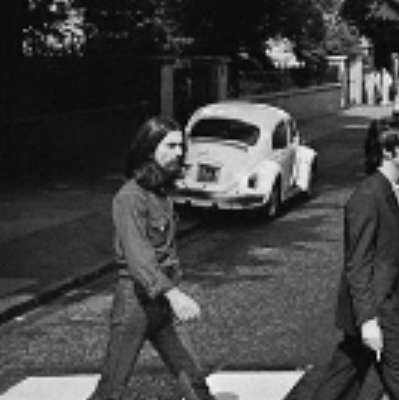
\includegraphics[scale=0.5]{imagenes/imagen4informe.png}
    \caption{Fracci\'on Imagen 4 - Bilineal por bloques}
    \end{figure}

     \begin{figure}[H]
    \centering
    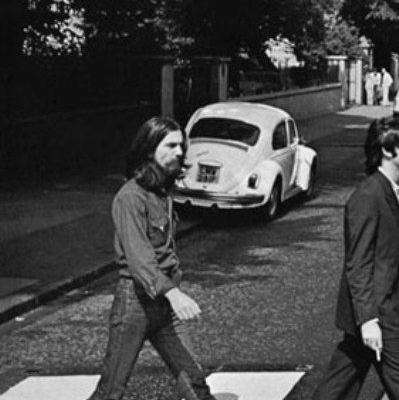
\includegraphics[scale=0.5]{imagenes/imagen4informeOriginal.png}
    \caption{Fracci\'on Imagen 4 - Orginal}
    \end{figure}

     \begin{figure}[H]
    \centering
    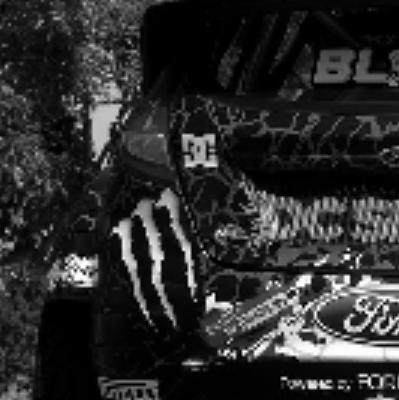
\includegraphics[scale=0.5]{imagenes/imagen5informe.png}
    \caption{Fracci\'on Imagen 5 - Bilineal por bloques}
    \end{figure}

     \begin{figure}[H]
    \centering
    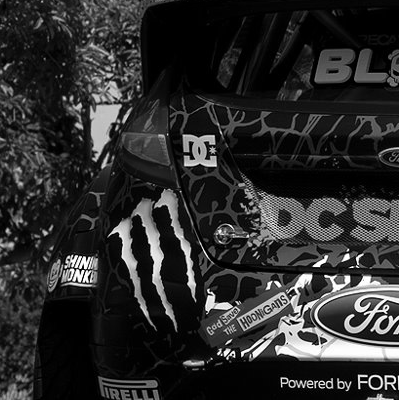
\includegraphics[scale=0.5]{imagenes/imagen5informeOriginal.png}
    \caption{Fracci\'on Imagen 5 - Orginal}
    \end{figure}

Tambien es notable que el m\'etodo con la variante de ignorar un pixel, en las imagenes que varia el color seguido, deja m\'as detalles especiales de lo que esperabamos, como una imagen despixelada, o con franjas blancas. En cambio en las que no var\'ia el color seguido, deja imagenes aceptables. En la siguiente comparaci\'on se observa lo recientemente detallado.\\
 \begin{figure}[H]
    \centering
    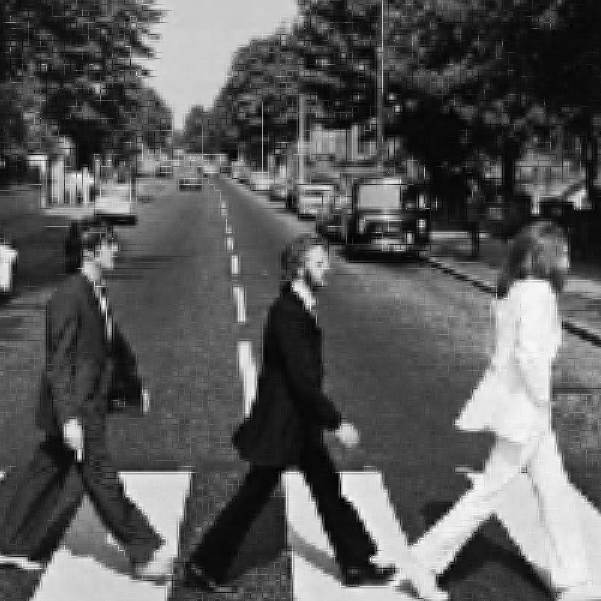
\includegraphics[scale=0.5]{imagenes/imagen4informe2.png}
    \caption{Fracci\'on Imagen 4 - Bilineal ignorando un pixel}
    \end{figure}

     \begin{figure}[H]
    \centering
    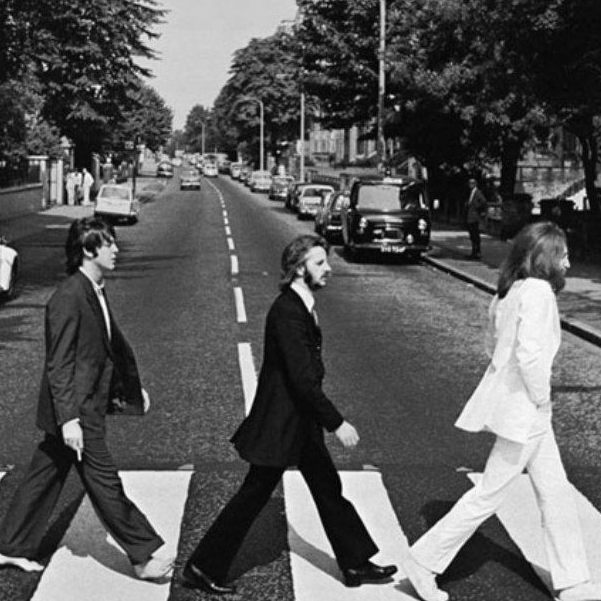
\includegraphics[scale=0.5]{imagenes/imagen4informe2Original.png}
    \caption{Fracci\'on Imagen 4 - Orginal}
    \end{figure}

     \begin{figure}[H]
    \centering
    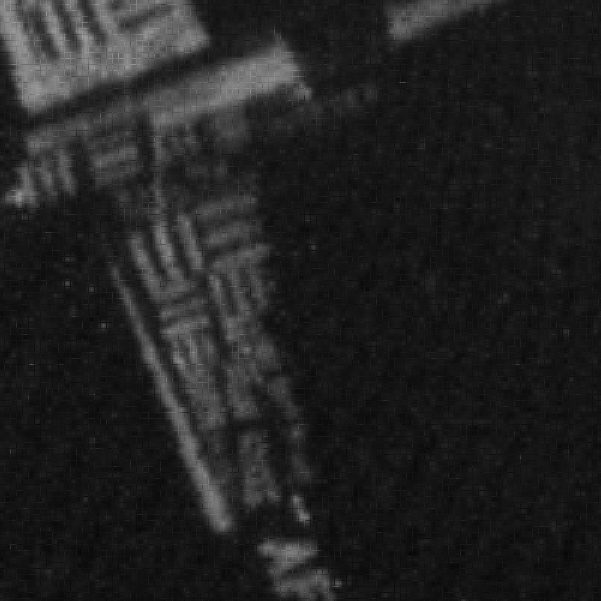
\includegraphics[scale=0.5]{imagenes/imagen2informe.png}
    \caption{Fracci\'on Imagen 2 - Bilineal por bloques}
    \end{figure}

     \begin{figure}[H]
    \centering
    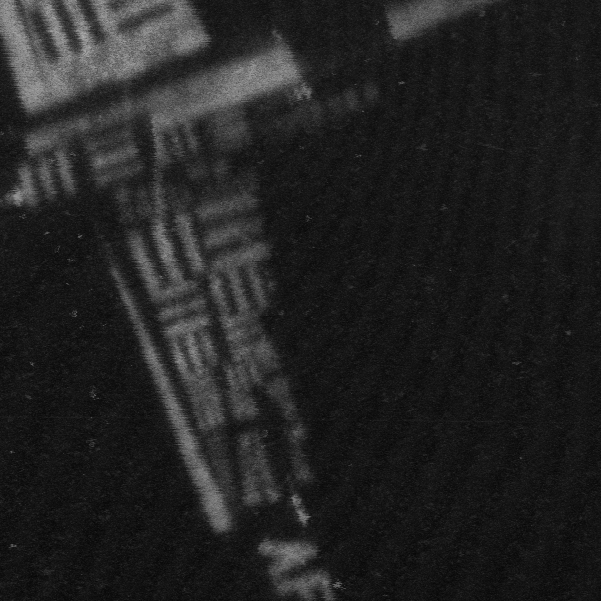
\includegraphics[scale=0.5]{imagenes/imagen2informeOriginal.png}
    \caption{Fracci\'on Imagen 2 - Orginal}
    \end{figure}
Comparando las variantes original, por diagonal y por bloques sobre cada una de las imagen, no se noto diferencias visibles al sentido humano comparando cada una de ellas, es decir comparando la misma foto pero con diferentes variantes.
\section{Discusion}
\subsection{Metodo Bilineal}
 Con las im\'agenes donde no hab\'ia cambios tan seguidos de colores, se pudo verificar que la variante de ignorar un pixel, retorno un valor similar de PSNR, con diferencias de 1 0 2 puntos en relaci\'on a las otras variantes. Nunca se obtuvo mejor valor de PSNR.
 En cuanto con las im\'agenes que si tenian cambios seguidos de color, el valor de PSNR dio muy por debajo de lo que dieron las otras variantes, llegando a diferencias de entre 4 y 6 puntos. Ademas se encontraron artifacts muy notorios en las im\'agenes como los expuestos en la secci\'on de resultados.\\
 Tambien los resultados mostraron que la variante original y la de por bloques, casi devolvieron similares valores de PSNR, con minimas diferencias, siempre obteniendo mayor valor la variante por bloques. Suponiamos que iban a dar similares pero que la variante original iba a dar siempre mejor que por bloques debido a que en la implementaci\'on se realizan menos casteos de variables y eso podria haber arrastrado errores de precisi\'on.\\
 En cuanto a los valores de PSNR de la variante de diagonales, siempre obtuvimos valores con diferencias de a lo sumo 1 punto, lo que marcar\'ia que las im\'agenes elegidas posiblemente no tengan una continuidad diagonal de color en todos los sectores.\\
 Para destacar es que los resultados arrojaron que a medida que el k aumenta, si la imagen posee bastantes cambios abruptos de colores, se obtendr\'an imagenes con menos calidad objetiva y subjetiva.\\
 Para finalizar con el estudio de este metodo, concluimos que la mejor variante en cuanto tiempo, calidad objetiva y calidad subjetiva es la variante por bloques.



\section{Conclusiones}

\begin{thebibliography}{abbrvnat}
\bibitem{burden} Burden R. L., Faires J.D.- Numerical Analysis
\end{thebibliography}

\end{document}

